\section{Appendix}

\subsection{Appendix A: Basics from Molecular Biology} \label{fundamentalsA}

\subsubsection{Genome Sequences} \label{fundamentalsAa}

\begin{wrapfigure}{R}{6cm}
	\centering
	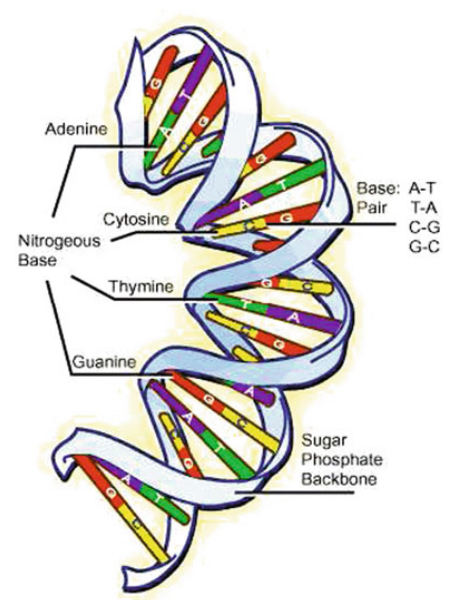
\includegraphics[width=0.9\linewidth]{figures/dnaDoubleHelix.png}
	\caption{\ac{DNA} double helix \cite[p. 8]{10.5555/1965281}}
	\label{dna_double_helix}
\end{wrapfigure}

The human genome is encoded as \ac{DNA}. The \ac{DNA} carries genetic instructions on how \ac{DNA} based organisms develop and behave. It is structured as a double helix and consists of two nucleotide pair combinations: adenine (A), thymine (T) and cytosine (C), guanine (G). \cite[p. 8]{10.5555/1965281}

%\begin{figure}[ht]
%	\centering
%	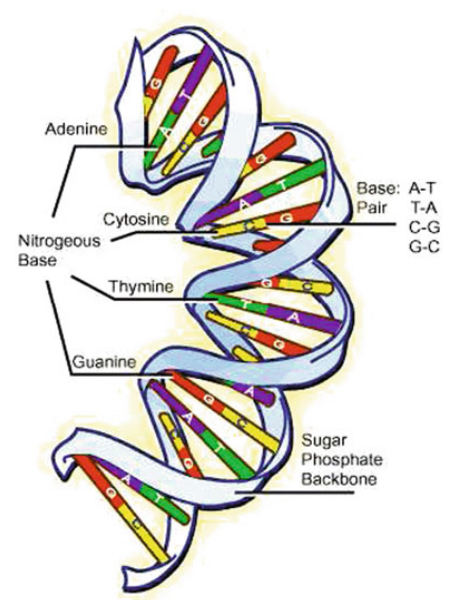
\includegraphics[width=0.35\linewidth]{figures/dnaDoubleHelix.png}
%	\caption{\ac{DNA} double helix \cite[p. 8]{10.5555/1965281}}
%	\label{dna_double_helix}
%\end{figure}

\subsubsection{Protein Biosynthesis} \label{fundamentalsAb}

The protein biosynthesis (also known as the central dogma of molecular biology) describes how proteins are produced based on \ac{DNA} sequences. The proteins then produce characteristics (e.g. human hair color). So the \ac{DNA} directly influences which human characteristics are developed. \cite[p. 6]{schererStatisticalGeneticsGenetic2021}

The process of protein biosynthesis can be seen in \autoref{protein_biosynthesis}. The single steps are described in the following:
\begin{enumerate}
	\item Transcription: The \ac{DNA} is transcribed by the RNA-Polymerase into pre-messenger RNA. As part of this process, the nucleotide thymine is replaced by uracil (U). \cite[p. 9]{schererStatisticalGeneticsGenetic2021}
	\item mRNA Processing: The pre-messenger RNA is transformed into the messenger RNA by removing the non-coding regions (introns). So the main difference between \ac{DNA} and \ac{RNA} is that the \ac{DNA} is structured as a double helix, whereas the \ac{RNA} consists of a single strain. \cite[p. 9]{schererStatisticalGeneticsGenetic2021}
	\item Translation: Ribosomes translate the mRNA into amino acids. Three nucleotides (one codon) decode one amino acid. The matching which codons decode for which amino acid can be seen in \autoref{genetic_code}. \cite[p. 9]{schererStatisticalGeneticsGenetic2021}
\end{enumerate}

\begin{figure}[ht!]
	\centering
	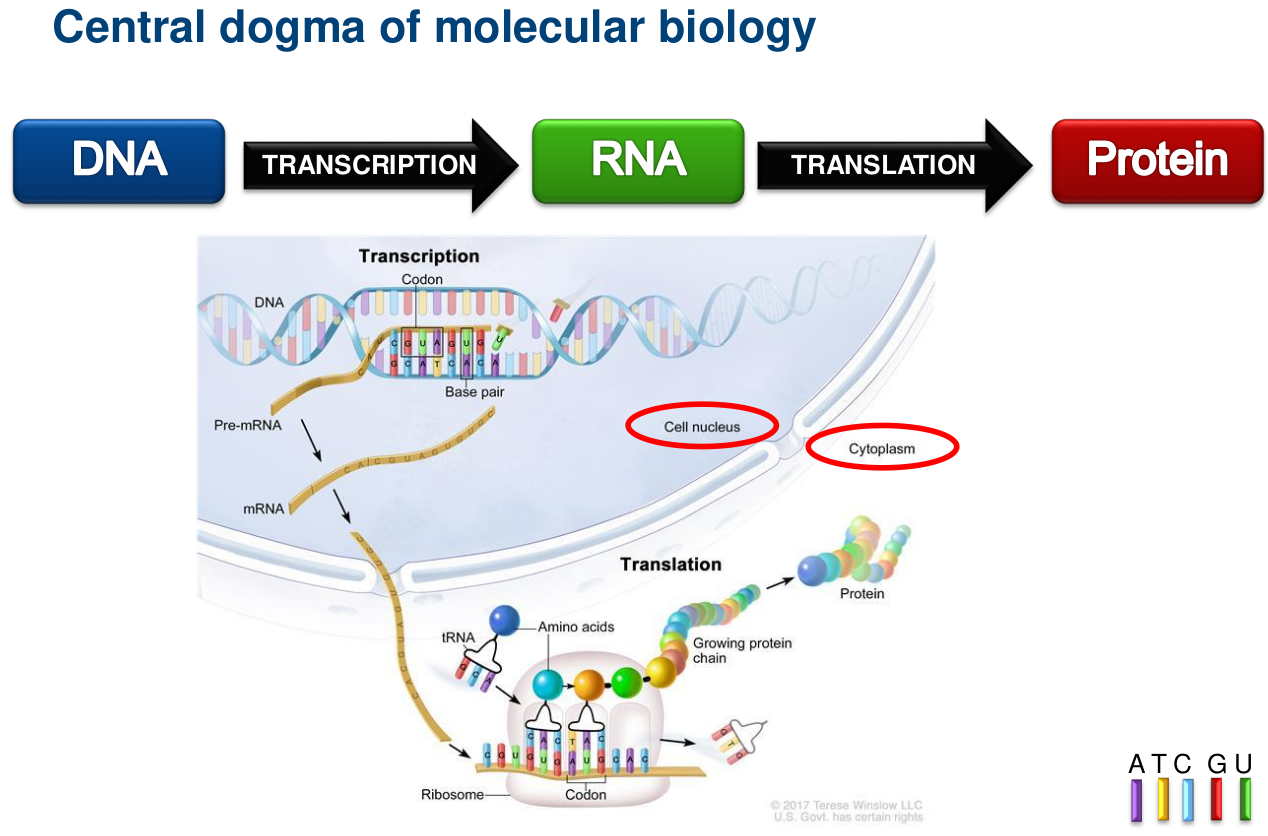
\includegraphics[width=0.9\linewidth]{figures/dogmaMolecularBiology.png}
	\caption{Protein biosynthesis \cite[p. 6]{schererStatisticalGeneticsGenetic2021}}
	\label{protein_biosynthesis}
\end{figure}

\begin{figure}[ht!]
	\centering
	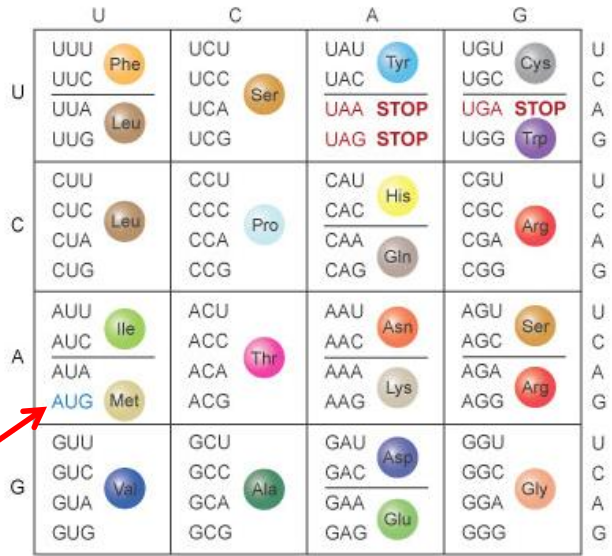
\includegraphics[width=0.5\linewidth]{figures/geneticCode.png}
	\caption{Genetic code \cite[p. 10]{schererStatisticalGeneticsGenetic2021}}
	\label{genetic_code}
\end{figure}


\subsubsection{Structure of \ac{SARS-CoV-2}} \label{fundamentalsAc}

\ac{RNA} based viruses (like \ac{SARS-CoV-2}) use \ac{RNA} to encode their genetic information. That means that the genetic information is present as a single strained \ac{RNA} sequence. This sequence contains for example the information on which proteins form the surface structure of the SARS-CoV-2 virus and how this surface looks like. \cite{NAQVI2020165878}

Based on Naqvi et al. \cite{NAQVI2020165878} the four proteins forming \ac{SARS-CoV-2} are:
\begin{itemize}
	\item spike (S)
	\item envelope (E)
	\item membrane (M)
	\item nucleocapsid (N)
\end{itemize}

A structural representation of \ac{SARS-CoV-2} and a host cell is visualized in \autoref{sarscov2_structure}. \cite{NAQVI2020165878}

\begin{figure}[ht]
	\centering
	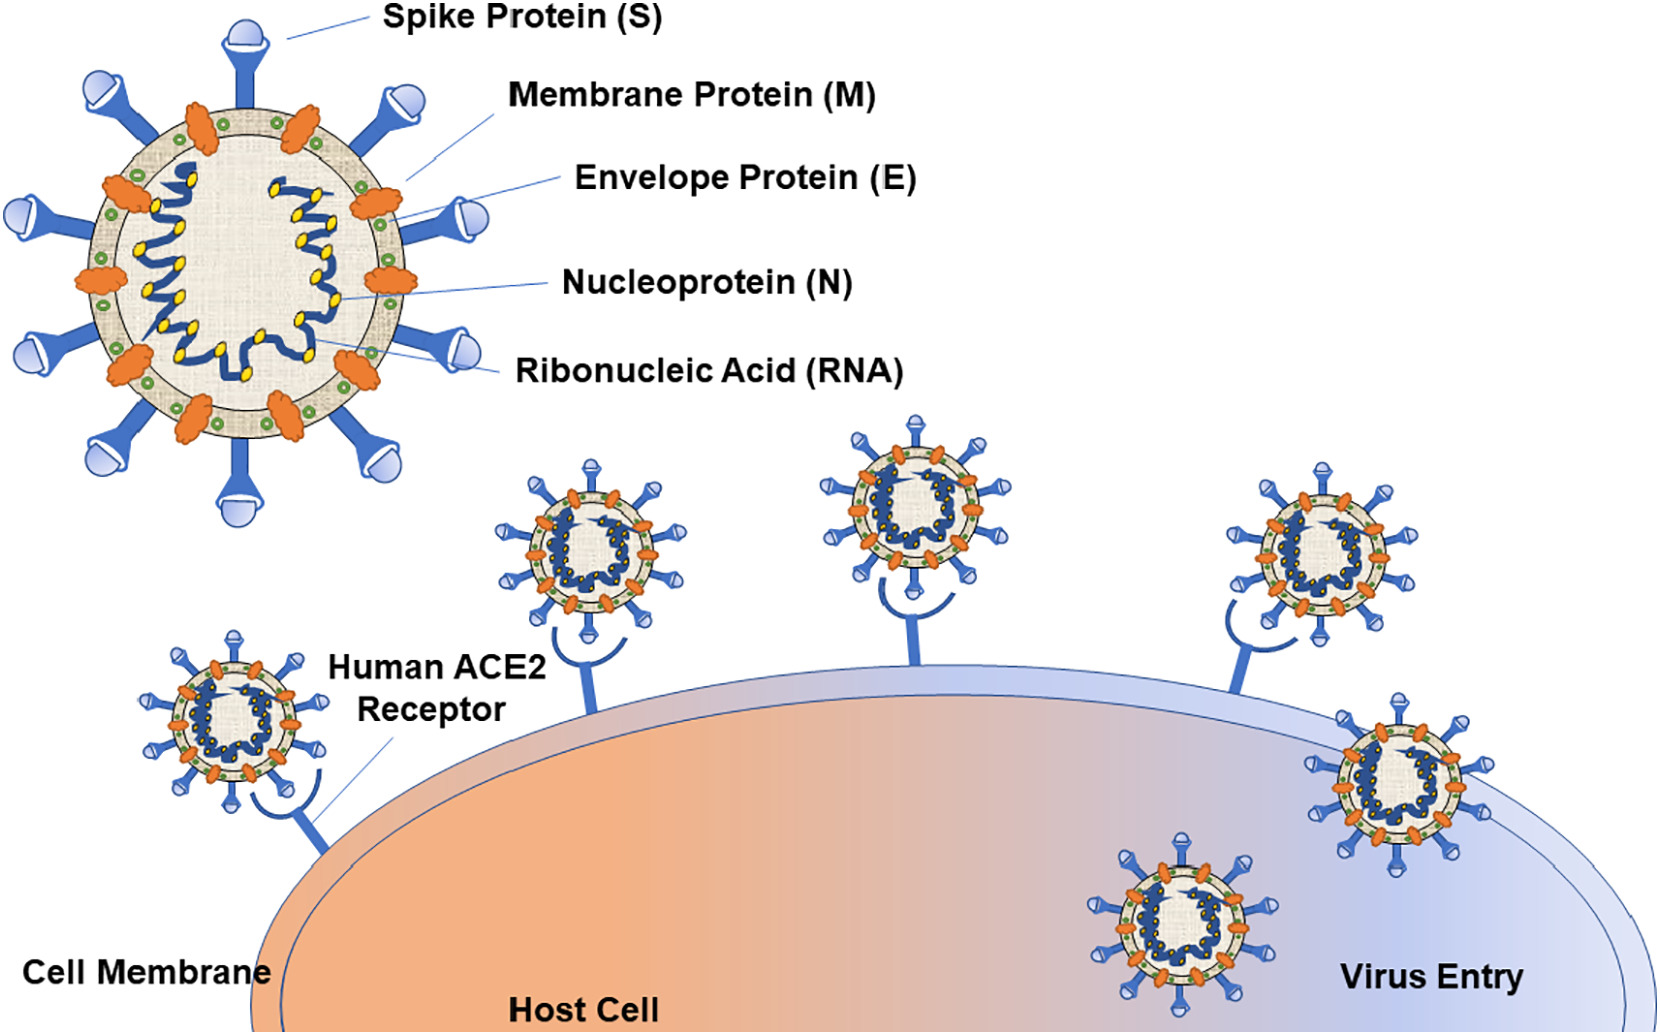
\includegraphics[width=0.8\linewidth]{figures/SARS-CoV-2Structure.jpg}
	\caption{SARS-CoV-2 structure \cite[p. 2]{NAQVI2020165878}}
	\label{sarscov2_structure}
\end{figure}

Furthermore \autoref{sarscov2_structure} shows the \ac{RNA} in the center. The \ac{SARS-CoV-2} \ac{RNA} consists of about 30,000 nucleotides, which belong to different subgroups, as shown in \autoref{sarscov2GenomeStructure}. 
Padded by a 5' \ac{UTR} at the beginning and a 3' \ac{UTR} in the end (\ac{UTR} are markers for the beginning and the end of protein-coding sequences), the middle part contains 12 functional \ac{ORF}, which contain the four coding regions for the proteins S, E, M and N. 

\begin{figure}[ht]
	\centering
	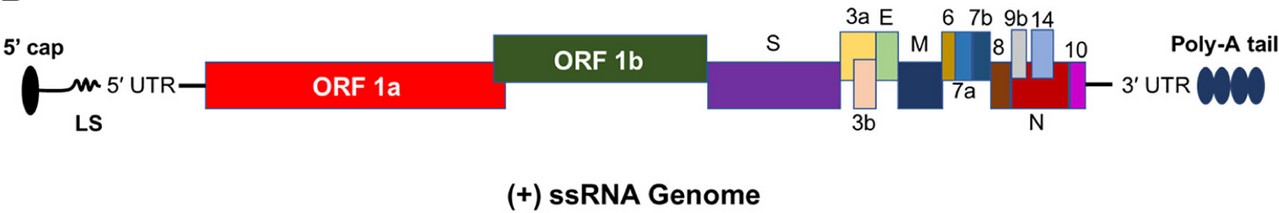
\includegraphics[width=1.0\linewidth]{figures/sarscov2GenomeStructure.png}
	\caption{\ac{SARS-CoV-2} genome structure \cite[p. 3]{NAQVI2020165878}}
	\label{sarscov2GenomeStructure}
\end{figure}

\subsubsection{Relationships between Biological Objects} \label{fundamentalsAd}

One main question in biology is to determine relationships between objects, such as species or genome sequences. The observed objects are called taxa. Most commonly used for determining these relationships is the phy\-lo\-ge\-ne\-tic analysis which generates a phy\-lo\-ge\-ne\-tic tree. In this phy\-lo\-ge\-ne\-tic tree, each leaf node corresponds to exactly one taxon. The inner nodes of the tree are the inferred hypothetical ancestors, which are no taxa. The relatedness between different taxa can be evaluated by their distance. \cite{böckenhauer2013algorithmische}

\autoref{examplePhylogeneticTree} shows an example phylogenetic tree calculated based on the species genomes. On the right side, each leaf node (taxa) corresponds to one current species. From left to right one can see the inferred historical development from the ancestors to the current species. One can see, that Gorillas and Orangutans have earlier developed apart than the other species. Furthermore one can see, that the  Chimpanzees and Bonobos share a most recent common ancestor (inner node next to both). That is why they are more related to each other. \cite{mallawaarachchiMolecularPhylogeneticsUsing2018}

\begin{figure}[ht]
	\centering
	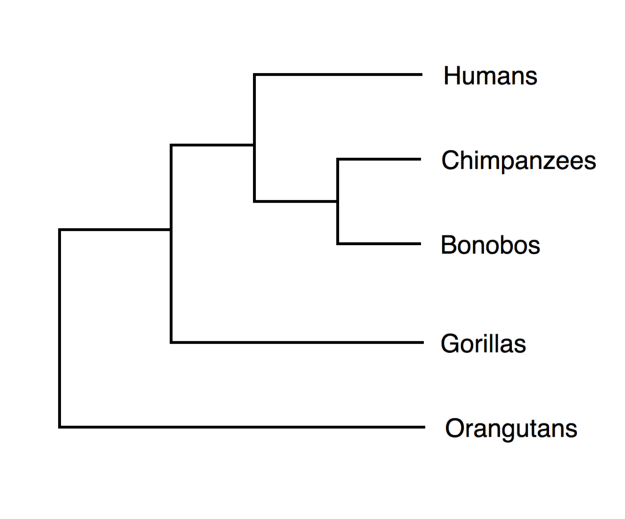
\includegraphics[width=0.5\linewidth]{figures/examplePhylogeneticTree.png}
	\caption{Example phylogenetic tree \cite{mallawaarachchiMolecularPhylogeneticsUsing2018}}
	\label{examplePhylogeneticTree}
\end{figure}

\newpage